\chapter{Interface}
\label{ch:interface}

The interface was designed so that the steps to convert a Z specification to a
fully proven specification would be easier to complete by the user. It made the
\gls{zmath} process more user friendly then by just typing commands in a
terminal. Full details for the user interface and all its functions can be found
in Mihaylova's user guide \cite{zmathuser}. This chapter only explains the process
needed to translate a specification into a full proof, other steps such as
writing the specification in the first place and outputting pdf using the
interface can be found in the manual.

\section{Inserting a specification}
To use the \gls{zmath} framework through the interface the user can download the
files from \cite{zmathweb} then using a terminal run the interface program by
typing \newline \verb|python Interface.py|, figure \ref{fig:startinterface}
shows an example of this.

\begin{figure}[H]
    \centering
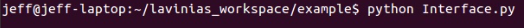
\includegraphics[scale=0.8]{Figures/Interface/startinterface.png}
\caption{Example of how to start the interface for the \gls{zmath} framework using the terminal. \label{fig:startinterface}}
\end{figure}

An example of the interface can be seen in figure \ref{fig:openspec}. Depending
on the operating system the interface may look slightly different however the
main panels and buttons will be the same. The main menu bar is at the top left
had side and the main panel is on the left. There is a messages panel on the
right top side which displays any messages when checking for correctness and
converting to skeletons. To check a specification the user can click \emph{file}
then \emph{open} from the main menu as shown in figure \ref{fig:openspec}.

\begin{figure}[H]
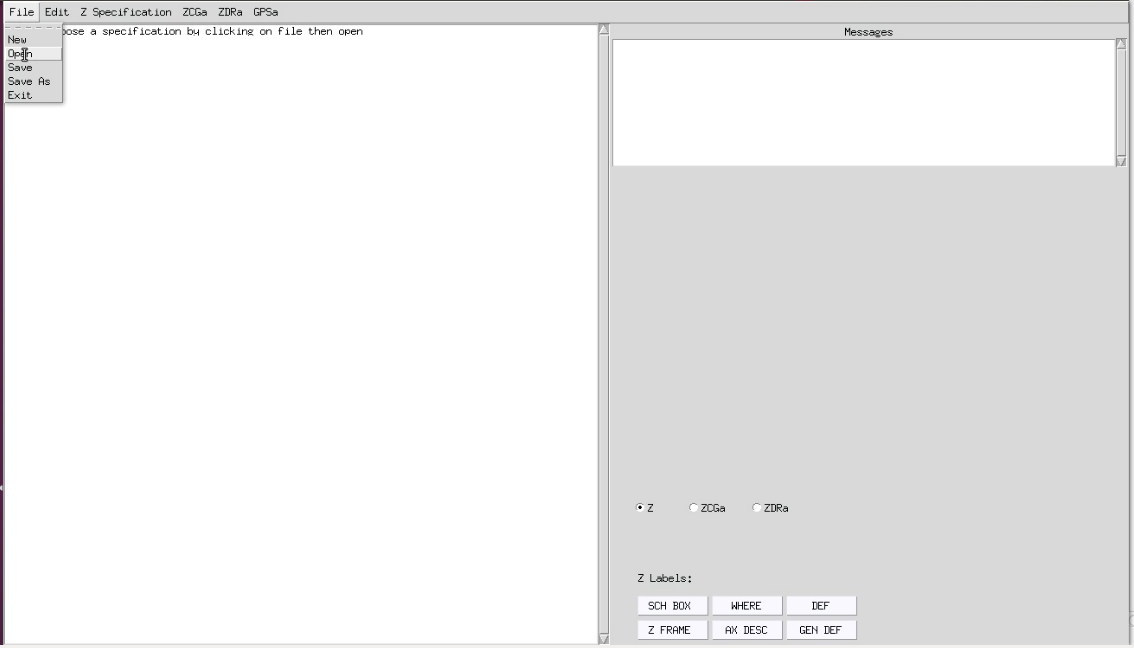
\includegraphics[scale=0.4]{Figures/Interface/openspec.png}
\caption{This figure shows the steps to open an existing specification to be imported into the user interface. \label{fig:openspec}}
\end{figure}

A pop up box appears asking the user to locate the specification they would like
to translate. An example of the pop up box is shown in figure
\ref{fig:choosespec}. 

\begin{figure}[H]
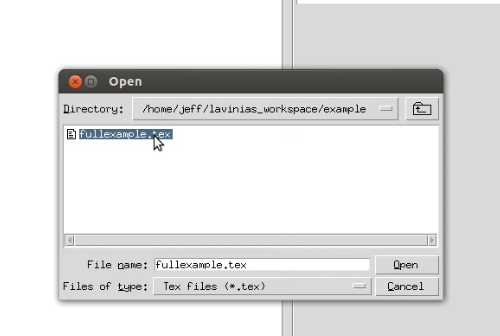
\includegraphics[scale=0.8]{Figures/Interface/choosespec.png}
\caption{This figure shows the pop  up  window that comes up when a user is asked which specification they wish to insert. In our example we would like to import a file named "fullexample.tex". \label{fig:choosespec}}
\end{figure}

Once a specification has been chosen then the specification should appear in the
panel on the left hand side. Figure \ref{fig:specinserted} shows an example of
this. Note that no messages appear yet in the messages box.

\begin{figure}[H]
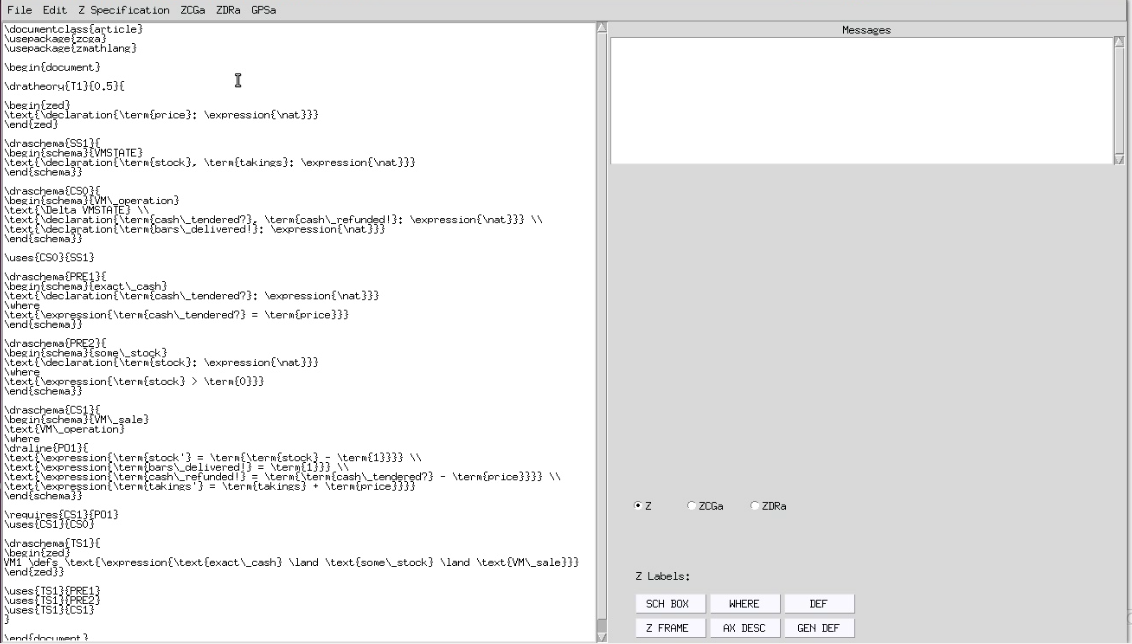
\includegraphics[scale=0.37]{Figures/Interface/specinserted.png}
\caption{This figure shows an imported in the user interface which is shown in the main panel on the left. \label{fig:specinserted}}
\end{figure}

\section{Checking ZCGa}
To then check for \gls{zcga} correctness the specification loaded into the
interface must be \gls{zcga} annotated.

\begin{figure}[H]
\centering
\begin{minipage}{0.45\textwidth}
\centering
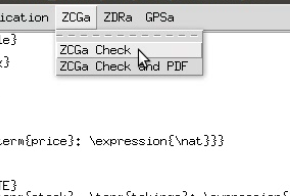
\includegraphics[scale=0.6]{Figures/Interface/zcgacheck.png}
\end{minipage}\hfill
\begin{minipage}{0.45\textwidth}
\centering
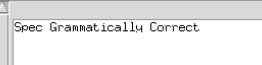
\includegraphics[scale=0.7]{Figures/Interface/zcgacorrect.png}
\end{minipage}
\caption{An example of how to check the specification for ZCGa correctness (left) and the message which appears when the specification is ZCGa correct (right).  \label{fig:zchecheck}}
\end{figure}

To check for \gls{zcga} correctness the user can click on the \emph{zcga} button
from the top menu and then click on \emph{Zcga Check}. If the specification is
grammatically correct then a message appears in the message box in the top right
of the interface (n see figure \ref{fig:zchecheck}).

\section{Checking ZDRa}

To check for \gls{zdra} correctness the specification loaded into the interface
must be labelled with \gls{zdra} annotations (this can be with or without
\gls{zcga} annotations).

\begin{figure}[H]
\centering
\begin{minipage}{0.4\textwidth}
\centering
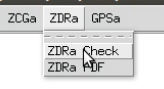
\includegraphics[scale=0.7]{Figures/Interface/zdracheck.png}
\end{minipage}\hfill
\begin{minipage}{0.6\textwidth}
\centering
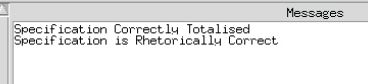
\includegraphics[scale=0.6]{Figures/Interface/zdracorrect.png}
\end{minipage}
\caption{An example of how to check the specification for ZDRa correctness (left) and the message which appears when the specification is ZDRa correct.  \label{fig:zdracheck}}
\end{figure}

To check for \gls{zdra} correctness the user can click on the \emph{ZDRa} button
in the top menu of the interface and then on the \emph{Zdra Check} button. If
the specification is \gls{zdra} correct and the specification has been correctly
totalised then a message confirming this appears in the message box. Figure
\ref{fig:zdracheck} shows both of these actions.

\section{Skeletons}

The user may also want to create a general proof skeleton, Isabelle skeleton and
fill in the Isabelle skeleton using the Interface. This section explains how
this may be done.

\subsection{General Proof Skeleton}

To create a general proof skeleton from the users \gls{zdra} annotated and
correct specification. The user will need to input their specification into the
interface, check the specification for \gls{zdra} correctness then click on the
\emph{GPSa} button in the top menu and choose \emph{Proof Skeleton} from the
drop down menu. An example of this is shown in figure \ref{fig:gpsabutton}.

\begin{figure}[H]
\centering
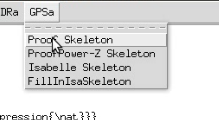
\includegraphics[scale=0.8]{Figures/Interface/proofskeleton.png}
\caption{This part of the user interface shows the steps to create a general proof skeleton from the users loaded specification.. \label{fig:gpsabutton}}
\end{figure}

A new file should then appear in the same folder as your \texttt{Interface.py}
program (see figure \ref{fig:gpsadoc}).

\begin{figure}[H]
\centering
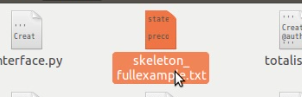
\includegraphics[scale=0.6]{Figures/Interface/skeletondoc.png}
\caption{A new file appears named skeleton in the same directory as the users specification. This is the automatically generated skeleton. \label{fig:gpsadoc}}
\end{figure}

The user may then open this file using an external text editor or they may view
it in the interface itself. When creating a general proof skeleton a message
appears in the Messages box saying \texttt{Skeleton Created}, a button also
appears underneath the message box saying \texttt{Show Skeleton} (see figure
\ref{fig:showskeleton}). By clicking on this new button the general proof
skeleton can be opened within the Interface. 

\subsection{Isabelle Skeleton}

After creating a general proof skeleton the user may want to take the
translation one step further and create an Isabelle proof skeleton. Again, to do
this the specification must be labelled with \gls{zdra} and be \gls{zdra}
correct. The user may then click on the \emph{GPSa} button in the top menu and
then the \emph{Isabelle Skeleton} button in the drop down menu as shown in
figure \ref{fig:converttoisa}.

\begin{figure}[H]
\centering
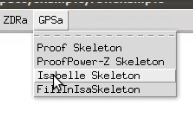
\includegraphics[scale=0.8]{Figures/Interface/isskeleton.png}
\caption{To create an Isabelle skeleton then `\textit{Isabelle Skeleton}' should be selected from the GPSa sub menu on the user interface. \label{fig:converttoisa}}
\end{figure}

If all is correct a message saying \texttt{Isabelle Skeleton Created} and a new
button should appear under the message box with the text \texttt{Show Isabelle
Skeleton} as seen in figure \ref{fig:showskeleton}. A new file will be produced
and automatically saved in the same directory as the interface with a
\emph{.thy} extension.

\begin{figure}[H]
\centering
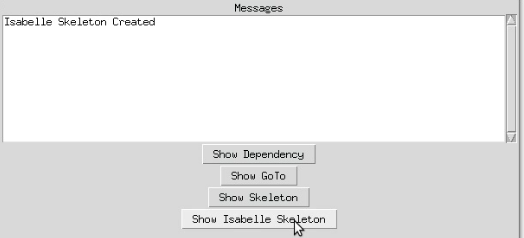
\includegraphics[scale=0.7]{Figures/Interface/showsaskeleton.png}
\caption{New buttons which appear on the right hand side of the interface if the user chooses to create a general proof skeleton or an Isabelle skeleton. \label{fig:showskeleton}}
\end{figure}

The user may then open the Isabelle skeleton using an external text editor such
as Jedit or Isabelle itself or they may choose to open the Isabelle Skeleton
within the interface by clicking on the \texttt{Show Isabelle Skeleton Button}.
An example of a pop-up window showing the Isabelle skeleton in the user
interface can be seen in figure \ref{fig:isaskelpopup}.

\begin{figure}[H]
\centering
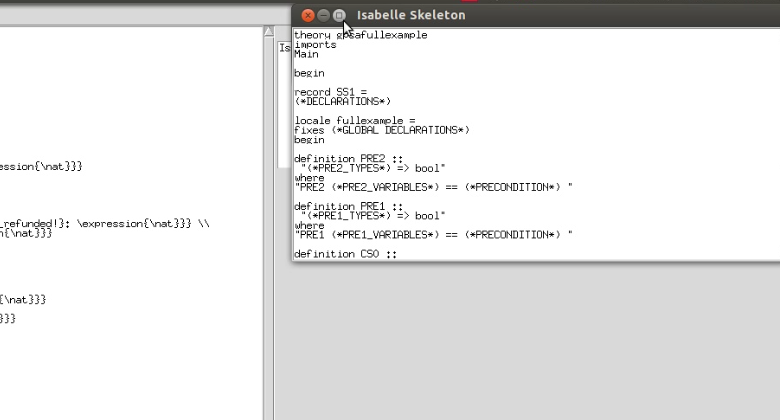
\includegraphics[scale=0.5]{Figures/Interface/isaskelpopup.png}
\caption{By clicking `\textit{Show Isabelle skeleton}' a box will be displayed in the user interface showing the isabelle skeleton. \label{fig:isaskelpopup}}
\end{figure}

The user may even wish to go as far as filling in the Isabelle skeleton. To do
this the Isabelle skeleton will need to be created first and the specification
loaded into the interface must also be annotated with \gls{zcga}. The user can
then click on \texttt{GPSa} in the top level menu and then
\texttt{FillInIsaSkeleton} (see figure \ref{fig:fillinisaskel}). If the skeleton
is not in the same directory as the interface or has been renamed then the
interface will ask for the user to locate the Isabelle skeleton in a similar way
to opening a specification (figure \ref{fig:choosespec}).

\begin{figure}[H]
\centering
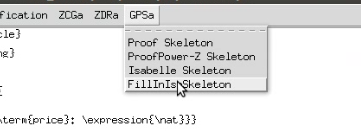
\includegraphics[scale=0.7]{Figures/Interface/fillinisaskel.png}
\caption{This figure shows the steps to automatically fill in the Isabelle skeleton. The user can choose the `\textit{FillInIsaSkeleton}' from the GPSa sub menu. \label{fig:fillinisaskel}}
\end{figure}

The user may then wish to open the filled-in isabelle skeleton externally or in
the interface the same was as they opened the skeleton in the previous step.

\section{Output messages which could occur}

Sometimes there is an error in any of the actions previously described in this
chapter. The message box not only tells the user what has been successful but it
also gives the user information if there has been some error in the action they
were trying. Table \ref{tab:uimessages} shows all the possible messages which
can appear in the message box along with an explanation about the message.

{\def\arraystretch{0.5}\tabcolsep=0.5pt
\begin{longtable}[H]{|l | l |}
\hline
\textbf{Text in message box} & \textbf{Explanation} \\
\hline
\hline
\verb|Specification Correctly| & All preconditions in the specification\\
\verb|Totalised| & have a totalising condition  \\
\hline
\verb|Warning! Specification not| & Not all preconditions have an alternative \\
\verb|correctly totalised| & output (skeleton can still be created) \\
& \textit{(see chapter \ref{ch:zdra})} \\
\hline
\verb|Specification is Rhetorically| & Specification is ZDRa correct \\
\verb|Correct| & \textit{(see chapter \ref{ch:zdra})} \\
\hline
\verb|Skeleton Created| & General proof skeleton has been successfully \\
& created \\
\hline
\verb|Isabelle Skeleton Created| & Isabelle skeleton has been successfully
created \\
\hline
\verb|Isabelle Skeleton successfully| & Isabelle proof skeleton has been \\
\verb|filled in| & filled in using ZCGa text \\
\hline
\verb|Please convert specification| & Covert the specification into an  \\
\verb|into Isabelle Skeleton first| & Isabelle skeleton first before filling it
in \\
& \textit{(see chapter \ref{ch:skeletons})} \\
\hline
\verb|Please select your isabelle| & Please locate the Isabelle skeleton\\
\verb|skeleton:| & which you wish to be filled in \textit{(see chapter
\ref{ch:skeletons})}\\
\hline
\verb|Please convert specification| & Can not find the \\
\verb|into GPSa first| & general proof skeleton \textit{(see chapter
\ref{ch:skeletons})}\\
\hline
\verb|Loops in reasoning| & Specification is not ZDRa correct \\
\verb|Can not create Skeleton| & and the skeleton can not be created \\
& \textit{(see chapter \ref{ch:zdra})}\\
\hline
\verb|Spec Grammatically Correct| & The specification has passed ZCGa checker \\
\hline
\verb|Spec Grammatically Incorrect|& The specification has failed ZCGa
correctness\\
\verb|Number of errors: 2| & and has 2 errors \textit{(see chapter
\ref{ch:zcga})}\\
\hline 
\caption{Messages which could appear in the user interface and their meanings.}
\label{tab:uimessages}
\end{longtable}
}

The user interface allows the users to create, import and edit a specification. It allows the
user to annotate their specification and check for ZCGa correctness. The user may also use the
interface to annotate and check for ZDRa correctness. The GPSa, Isabelle skeleton, dependency 
and GoTo may also be created via the user interface. The only part which currently may not be
done via the user interface is the final proofs in Isabelle. Here the user will need to complete
 the proof of their formal specification via the Isabelle user interface or another program 
 which can parse Isabelle. Future work on ZMathLang may include add on an Isabelle plug-in to 
 the ZMathLang user interface.
 The user will only need to use the terminal to start the ZMathLang user interface. All other
  steps are done via the ZMathLang or Isabelle interface (in the case of the final step).

\section{Conclusion}
This chapter has described how a user of the \gls{zmath} framework can use the
implemented user interface to assist them with checking for grammatical and
rhetorical correctness. The user interface also gives a clear and easy way to
translate the specification into a general proof skeleton, Isabelle skeleton and
filling in the Isabelle skeleton without using the user unfriendly terminal. The
interface also allows the user to view the documents automatically produced from
the annotated specification.
